
\section{Introduction to NN}


\begin{frame}{Neural Networks}
  
  \begin{figure}
    \centering
    \includegraphics[width=0.85\textwidth]{images/41377_2024_1590_Fig3_HTML.png}
  \end{figure}

\end{frame}

\begin{frame}{Networks for AND logic}
  \begin{multicols}{2}
\begin{center}
  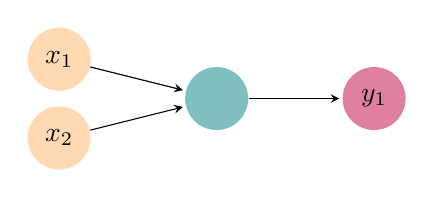
\begin{tikzpicture}[>=stealth]
% \centering
% Parameters
\def\inputnum{2}
\def\hiddennum{1}
\def\outputnum{1}

% Input Layer
\foreach \i in {1,...,\inputnum}
{
	\node[circle, minimum size=8mm, fill=orange!30] 
		(Input-\i) at (2,-\i) {$x_{\i}$};
}

% Hidden Layer
\foreach \i in {1,...,\hiddennum}
{
	\node[circle, minimum size=8mm, fill=teal!50,
		yshift=(\hiddennum-\inputnum)*5 mm]
		(Hidden-\i) at (4,-\i) {};
}

% Output Layer
\foreach \i in {1,...,\outputnum}
{
	\node[circle, minimum size=8mm, fill=purple!50,
		yshift=(\outputnum-\inputnum)*5 mm]
		(Output-\i) at (6,-\i) {$y_{\i}$};
}

% Connect neurons In-Hidden
\foreach \i in {1,...,\inputnum}
{
	\foreach \j in {1,...,\hiddennum}
	{
		\draw[->, shorten >=1pt] (Input-\i) -- (Hidden-\j);	
	}
}

% Connect neurons Hidden-Out
\foreach \i in {1,...,\hiddennum}
{
	\foreach \j in {1,...,\outputnum}
	{
		\draw[->, shorten >=1pt] (Hidden-\i) -- (Output-\j);
	}
}
\end{tikzpicture}
$$ y_1 = f(w_1 x_1 + w_2 x_2 + b)$$


    \begin{table}[h!]
    % \centering
    \begin{tabular}{|c|c|c|}
      \hline
      $x_1$ & $x_2$ & $y_1= x_1\land x_2 $ \\ 
      \hline
      0 & 0 & 0 \\ 
      0 & 1 & 0 \\ 
      1 & 0 & 0 \\ 
      1 & 1 & 1 \\ 
      \hline
    \end{tabular}
   
  \end{table}


  \vspace{0.5cm}
  \pause
  $$f(x) = \frac{1}{1+e^{-x}}$$
  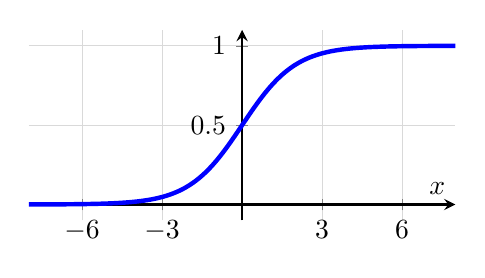
\begin{tikzpicture}
  \begin{axis}[
      axis lines = middle,
      samples = 200,
      domain = -8:8,
      width = 7cm,
      height = 4cm,
      xlabel = {$x$},
      % ylabel = {$f(x)$},
      ymin = -0.1, ymax = 1.1,
      grid = both,
      major grid style={gray!30},
      minor grid style={gray!10},
      thick,
      smooth,
      xtick={-6,-3,0,3,6},
      ytick={0,0.5,1}
    ]
    \addplot[blue, ultra thick, domain=-8:8]
      {1/(1+exp(-x))};
  \end{axis}
\end{tikzpicture}

\end{center}


  \end{multicols}

\end{frame}

\begin{frame}{Networks for AND logic}
\begin{equation*}
   y_1 = f(5.5 x_1 + 5.5 x_2 -8)
\end{equation*}
\begin{table}[h!]
\centering

\centering
\begin{tabular}{|c|c|c|c|c|}
\hline
$x_1$ & $x_2$ & Weighted Sum & $f(\text{sum})$ & Output \\ 
\hline
0 & 0 & -8.0 & 0.0003 & 0 \\ 
0 & 1 & -2.5 & 0.075  & 0 \\ 
1 & 0 & -2.5 & 0.075  & 0 \\ 
1 & 1 & 3.0  & 0.952  & 1 \\ 
\hline
\end{tabular}
\caption{Neural network output for AND operation.}

\hfill

\end{table}

\end{frame}

\begin{frame}{Training a Neural Networks}
\begin{center}
  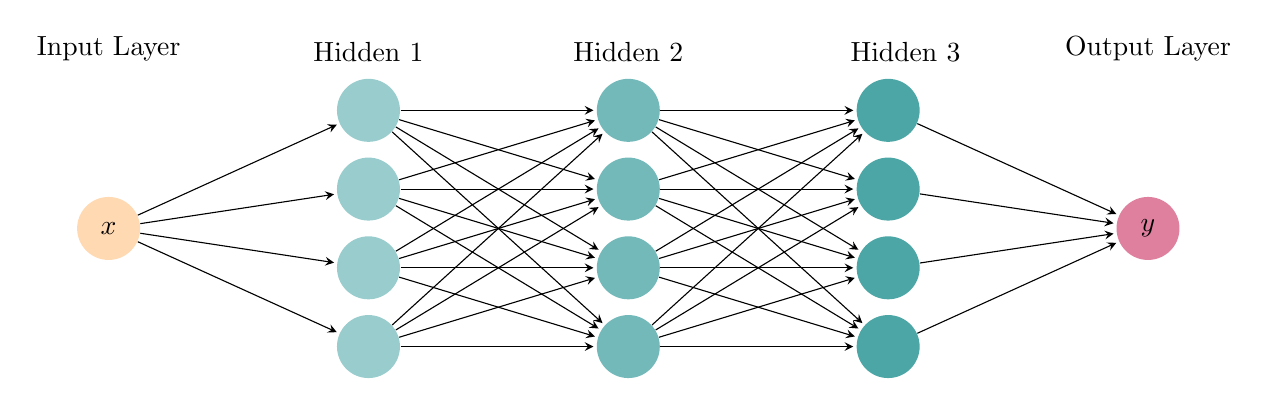
\begin{tikzpicture}[>=stealth, x=2.2cm, y=1cm]
\centering
% Parameters
\def\inputnum{1}
\def\hiddennum{4}
\def\outputnum{1}

% === Input Layer ===
\foreach \i in {1,...,\inputnum}{
  \node[circle, minimum size=8mm, fill=orange!30] 
    (Input-\i) at (0,-\i-1) {$x$};
}

% === Hidden Layer 1 ===
\foreach \i in {1,...,\hiddennum}{
  \node[circle, minimum size=8mm, fill=teal!40] 
    (HiddenA-\i) at (1.5,-\i + 0.5) {};
}

% === Hidden Layer 2 ===
\foreach \i in {1,...,\hiddennum}{
  \node[circle, minimum size=8mm, fill=teal!55] 
    (HiddenB-\i) at (3,-\i + 0.5) {};
}

% === Hidden Layer 3 ===
\foreach \i in {1,...,\hiddennum}{
  \node[circle, minimum size=8mm, fill=teal!70] 
    (HiddenC-\i) at (4.5,-\i + 0.5) {};
}

% === Output Layer ===
\foreach \i in {1,...,\outputnum}{
  \node[circle, minimum size=8mm, fill=purple!50]
    (Output-\i) at (6,-\i-1) {$y$};
}

% === Connections ===
% Input → Hidden 1
\foreach \i in {1,...,\inputnum}{
  \foreach \j in {1,...,\hiddennum}{
    \draw[->, shorten >=1pt] (Input-\i) -- (HiddenA-\j);
  }
}

% Hidden 1 → Hidden 2
\foreach \i in {1,...,\hiddennum}{
  \foreach \j in {1,...,\hiddennum}{
    \draw[->, shorten >=1pt] (HiddenA-\i) -- (HiddenB-\j);
  }
}

% Hidden 2 → Hidden 3
\foreach \i in {1,...,\hiddennum}{
  \foreach \j in {1,...,\hiddennum}{
    \draw[->, shorten >=1pt] (HiddenB-\i) -- (HiddenC-\j);
  }
}

% Hidden 3 → Output
\foreach \i in {1,...,\hiddennum}{
  \foreach \j in {1,...,\outputnum}{
    \draw[->, shorten >=1pt] (HiddenC-\i) -- (Output-\j);
  }
}

% === Labels ===
\node[above] at (0,0) {Input Layer};
\node[above] at (1.5,0) {Hidden 1};
\node[above] at (3,0) {Hidden 2};
\node[above] at (4.6,0) {Hidden 3};
\node[above] at (6,0) {Output Layer};
\end{tikzpicture}
\pause
$$ \text{Loss} = \frac{1}{N}\sum_{i}^{N}\left(y_{\text{nn}}(x_i)- y_{\text{true}}(x_i)\right)^2$$
\end{center}

\end{frame}

\begin{frame}{Training a Neural Networks}
  $$ \text{Cost} = \frac{1}{N}\sum_{i}^{N}\left(y_{\text{nn}}(x_i)- y_{\text{true}}(x_i)\right)^2$$

\begin{multicols}{2}
  \begin{center}
    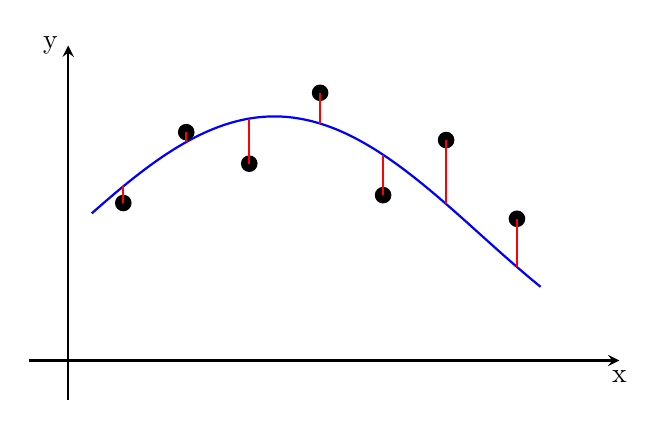
\begin{tikzpicture}[>=stealth, thick]

% ----- Axes -----
\draw[->] (-0.5,0) -- (7,0) node[below] {x};
\draw[->] (0,-0.5) -- (0,4) node[left] {y};

% ----- Regression curve -----
\draw[blue, thick, domain=0.3:6, smooth, samples=200]
  plot(\x,{1.6 + 1.5*sin(0.6*\x r)});

% ----- Data points -----
\foreach \x/\y in {0.7/2, 1.5/2.9, 2.3/2.5, 3.2/3.4, 4.0/2.1, 4.8/2.8, 5.7/1.8}{
  \fill[black] (\x,\y) circle (3pt);
}

% ----- Error lines (real error from curve to point) -----
\foreach \x/\y in {0.7/2, 1.5/2.9, 2.3/2.5, 3.2/3.4, 4.0/2.1, 4.8/2.8, 5.7/1.8}{
  \pgfmathsetmacro{\ycurve}{1.6 + 1.5*sin(0.6*\x r)}
  \draw[red] (\x,\y) -- (\x,\ycurve);
}

% ----- Optional: Label for "Error" -----
% \node[red, font=\bfseries] at (2.2,3.2) {Error};
\end{tikzpicture}
\pause
  \begin{figure}
    \centering
    \includegraphics[width=0.49\textwidth]{images/descent.jpg}
  \end{figure}

  \end{center}
  
\end{multicols}



\end{frame}
